\documentclass{article}
\usepackage[utf8]{inputenc} %кодировка
\usepackage[T2A]{fontenc}
\usepackage[english,russian]{babel} %русификатор 
\usepackage{mathtools} %библиотека матеши
\usepackage[left=1cm,right=1cm,top=2cm,bottom=2cm,bindingoffset=0cm]{geometry} %изменение отступов на листе
\usepackage{amsmath}
\usepackage{graphicx} %библиотека для графики и картинок
\graphicspath{}
\DeclareGraphicsExtensions{.pdf,.png,.jpg}
\usepackage{subcaption}
\usepackage{pgfplots}
\usepackage{float}
\usepackage{tikz}

\begin{document}
% НАЧАЛО ТИТУЛЬНОГО ЛИСТА
\begin{center}
    \Large
    Федеральное государственное автономное \\
    образовательное учреждение высшего образования \\ 
    «Научно-образовательная корпорация ИТМО»\\
    \vspace{0.5cm}
    \large
    Факультет программной инженерии и компьютерной техники \\
    Направление подготовки 09.03.04 Программная инженерия \\
    \vspace{1cm}
    \Large
    \textbf{Отчёт по домашней работе №1} \\
        По дисциплине Компьютерные сети ( семестр 6)\\
    \large
    \vspace{8cm}

    \begin{minipage}{.33\textwidth}
    \end{minipage}
    \hfill
    \begin{minipage}{.4\textwidth}
    
        \textbf{Студент}: \vspace{.1cm} \\
        \ Дениченко Александр P3312\\
        \textbf{Практик}:  \\
        \ Тропченко Андрей Александрович
    \end{minipage}
    \vfill
Санкт-Петербург\\ 2025 г.
\end{center}
\pagestyle{empty}
% КОНЕЦ ТИТУЛЬНОГО ЛИСТА 
\newpage
\pagestyle{plain}

\section*{Цель работы}
Изучение методов физического и логического кодирования,
используемых в цифровых сетях передачи данных.

\section{Формирование сообщения}

Исходное сообщение: Дениченко Александр Олегович
\\
В шестнадцатеричном коде: С4 E5 ED E8 F7 E5 ED EA EE C0 EB E5 EA F1 E0 ED E4 F0 СE EB E5 E3 EE E2 E8 F7
\\
В двоичном коде: 11000100 11100101 11101101 11101000 11110111 11100101 11101101 11101010 11101110 00100000 11000000 11101011 11100101 11101010 11110001 11100000 11101101 11100100 11110000 00100000 11001110 11101011 11100101 11100011 11101110 11100010 11101000 11110111
\\
Длина сообщения: 28 байт (224 бит)
\\
Пропускная способность канала связи: 100 Мбит/с 

\section{Физическое кодирование исходного сообщения}
\subsection{Манчестерский код}
Длительность битового интервала: $t_b = \frac{1}{C} = \frac{1}{100} = 0.01$
\\
Верхняя граница частот: $f_{up} = \frac{1}{t_b} = \frac{1}{0.01} = 100$ МГц
\\
Нижняя граница частот: $f_{down} = \frac{C}{2} = \frac{1}{0.01} = 50$ МГц
\\
Спектр сигнала: $S = f_{up} - f_{down} = 0.5C = 50$ МГц
\\
Среднее значение частоты в спектре передаваемого сигнала: $f_{avg} = \frac{f_{up}\cdot 252 + f_{down} \cdot 196}{448} = \frac{100\cdot 252 + 50 \cdot 196}{448} = 78.125$ МГц
\\
Среднеe арифметическое: $f_{1/2} = \frac{100 + 50}{2} = 75$ МГц
\\
В спектре сигнала незначительно преобладают высокие частоты: $f_{avg} > f_{1/2}$
\\
Ширина полосы пропускания: $F > 50 $МГц

\begin{center}
    \begin{tikzpicture}[scale=0.5]
        % Длина последовательности
        \def\bitlength{32}
    
        % Оси
        \draw[->] (0,0) -- (\bitlength+1,0) node[right] {Время};
        \draw[->] (0,-1.5) -- (0,1.5) node[above] {Уровень сигнала};
    
        % Битовая последовательность
        \foreach \x/\bit [remember=\bit as \prevbit (initially 0)] in {
            0/1, 1/1, 2/0, 3/0, 4/0, 5/1, 6/0, 7/0,
            8/1, 9/1, 10/1, 11/0, 12/0, 13/1, 14/0, 15/1,
            16/1, 17/1, 18/1, 19/0, 20/1, 21/1, 22/0, 23/1,
            24/1, 25/1, 26/1, 27/0, 28/1, 29/0, 30/0, 31/0}
        {
            \pgfmathtruncatemacro{\next}{\x+1}
            
            % Манчестерское кодирование
            \ifnum\bit=1
                \draw[thick] (\x,0.5) -- (\x+0.5,0.5);
                \draw[ultra thick, blue] (\x+0.5,0.5) -- (\x+0.5,-0.5);
                \draw[thick] (\x+0.5,-0.5) -- (\next,-0.5);
                \ifnum\prevbit=1
                    \draw[thick] (\x,0.5) -- (\x,-0.5);
                \fi
            \else
                \draw[thick] (\x,-0.5) -- (\x+0.5,-0.5);
                \draw[ultra thick, red] (\x+0.5,-0.5) -- (\x+0.5,0.5);
                \draw[thick] (\x+0.5,0.5) -- (\next,0.5);
                \ifnum\prevbit=0
                    \draw[thick] (\x,0.5) -- (\x,-0.5);
                \fi
            \fi
    
            % Разделительные линии
            \draw[dashed] (\next,1) -- (\next,-1);
    
            % Подпись битов
            \node[below] at (\x+0.5,-0.8) {\bit};
        }
    \end{tikzpicture}
\end{center}

\subsection{Потенциальный код без возврата к нулю}
Верхняя граница частот: $T=2t$, $t=\frac{1}{C}$, $f_{up} = \frac{C}{2} = \frac{100}{2} = 50$ МГц
\\
Максимальная подпоследовательность единиц - 6 и нулей - 6, тогда

нижняя граница частот: $f_{down} = \frac{C}{12} = 8.33$ МГц
\\
Спектр сигнала: $S = f_{up} - f_{down} = 50 - 8.33 = 41.67$ МГц
\\
Среднее значение частоты: $f_{avg} = \frac{(46 \cdot f_0/1 + 14 \cdot 2 \cdot f_0/2 + 18 \cdot 3 \cdot f_0/3 + 12 \cdot 4 \cdot f_0/4 + 6 \cdot 5 \cdot f_0/5 + 3 \cdot 6 \cdot f_0/6)}{224} =22.1$ МГц, где $f_0 = \frac{C}{2}$ (частота основной гармоники)
\\
Среднеe арифметическое: $f_{1/2} = \frac{50 + 8.33}{2} = 29.165$ МГц
\\
В спектре сигнала незначительно преобладают низкие частоты: $f_{avg} < f_{1/2}$
\\
Ширина полосы пропускания: $F > 41.67 $МГц

\begin{center}
    \begin{tikzpicture}[scale=0.5]
        % Длина последовательности
        \def\bitlength{32}
    
        % Оси
        \draw[->] (0,0) -- (\bitlength+1,0) node[right] {Время};
        \draw[->] (0,-1.5) -- (0,1.5) node[above] {Уровень сигнала};
    
        % Битовая последовательность
        \foreach \x/\bit [remember=\bit as \prevbit (initially 0)] in {
            0/1, 1/1, 2/0, 3/0, 4/0, 5/1, 6/0, 7/0,
            8/1, 9/1, 10/1, 11/0, 12/0, 13/1, 14/0, 15/1,
            16/1, 17/1, 18/1, 19/0, 20/1, 21/1, 22/0, 23/1,
            24/1, 25/1, 26/1, 27/0, 28/1, 29/0, 30/0, 31/0}
        {
            \pgfmathtruncatemacro{\next}{\x+1}
            
            \ifnum\bit=1
                \draw[ultra thick, blue] (\x,0.5) -- (\x+1,0.5);
                \ifnum\prevbit=0
                    \draw[thick] (\x,0.5) -- (\x,-0.5);
                \fi
            \else
                \draw[ultra thick, red] (\x,-0.5) -- (\x+1,-0.5);
                \ifnum\prevbit=1
                    \draw[thick] (\x,0.5) -- (\x,-0.5);
                \fi
            \fi
    
            % Разделительные линии
            \draw[dashed] (\next,1) -- (\next,-1);
    
            % Подпись битов
            \node[below] at (\x+0.5,-0.8) {\bit};
        }
    \end{tikzpicture}
\end{center}

\subsection{Биполярный импульсный код (код с возвратом к нулю)}
Верхняя граница частот: $f_{up} = C = 100$ МГц
\\
Нижняя граница частот: $f_{down} = \frac{C}{4} = 25$ МГц
\\
Спектр сигнала: $S = f_{up} - f_{down} = 100 - 25 = 75$ МГц
\\
Среднее значение частоты: $f_{avg} = \frac{(363\cdot f_0 + 17\cdot f_0/2.5)}{380} = 97.31$ МГц
\\
Среднеe арифметическое: $f_{1/2} = \frac{100 + 25}{2} = 62.5$ МГц
\\
В спектре сигнала преобладают высокие частоты: $f_{avg} > f_{1/2}$
\\
Ширина полосы пропускания: $F > 75 $ МГц

\begin{center}
    \begin{tikzpicture}[scale=0.5]
        % Длина последовательности
        \def\bitlength{32}
    
        % Оси
        \draw[->] (0,0) -- (\bitlength+1,0) node[right] {Время};
        \draw[->] (0,-1.5) -- (0,1.5) node[above] {Уровень сигнала};
    
        % Битовая последовательность
        \foreach \x/\bit in {
            0/1, 1/1, 2/0, 3/0, 4/0, 5/1, 6/0, 7/0,
            8/1, 9/1, 10/1, 11/0, 12/0, 13/1, 14/0, 15/1,
            16/1, 17/1, 18/1, 19/0, 20/1, 21/1, 22/0, 23/1,
            24/1, 25/1, 26/1, 27/0, 28/1, 29/0, 30/0, 31/0}
        {
            \pgfmathtruncatemacro{\next}{\x+1}
            
            \ifnum\bit=1
                \draw[thick] (\x,0.5) -- (\x,0);
                \draw[ultra thick, blue] (\x,0.5) -- (\x+0.5,0.5);
                \draw[thick] (\x+0.5,0.5) -- (\x+0.5,0);
            \else
                \draw[thick] (\x,-0.5) -- (\x,0);
                \draw[ultra thick, red] (\x,-0.5) -- (\x+0.5,-0.5);
                \draw[thick] (\x+0.5,-0.5) -- (\x+0.5,0);
            \fi
    
            % Разделительные линии
            \draw[dashed] (\next,1) -- (\next,-1);
    
            % Подпись битов
            \node[below] at (\x+0.5,-0.8) {\bit};
        }
    \end{tikzpicture}
\end{center}

\subsection{Биполярное кодирование с чередующейся инверсией}
Верхняя граница частот: $f_{up} = \frac{C}{2} = 50$ МГц
\\
Нижняя граница частот: $f_{down} = \frac{C}{12} = 8.33$ МГц
\\
Спектр сигнала: $S = f_{up} - f_{down} = 41.67$ МГц
\\
Среднее значение частоты: $f_{avg} = \frac{(160 \cdot f_0/1 + 16 \cdot f_0/2 + 21 \cdot f_0/3 + 15 \cdot f_0/5 + 12 \cdot f_0/6)}{224} = 40.17$ МГц
\\
Среднеe арифметическое: $f_{1/2} = \frac{50 + 8.33}{2} = 29.165$ МГц
\\
В спектре сигнала преобладают высокие частоты: $f_{avg} > f_{1/2}$
\\
Ширина полосы пропускания: $F > 41.67$ МГц

\begin{center}
    \begin{tikzpicture}[scale=0.5]
        % Длина последовательности
        \def\bitlength{32}
    
        % Оси
        \draw[->] (0,0) -- (\bitlength+1,0) node[right] {Время};
        \draw[->] (0,-1.5) -- (0,1.5) node[above] {Уровень сигнала};
    
        % Битовая последовательность
        \def\lastlevel{-1} % Начинаем с отрицательного уровня для AMI
        \foreach \x/\bit in {
            0/1, 1/1, 2/0, 3/0, 4/0, 5/1, 6/0, 7/0,
            8/1, 9/1, 10/1, 11/0, 12/0, 13/1, 14/0, 15/1,
            16/1, 17/1, 18/1, 19/0, 20/1, 21/1, 22/0, 23/1,
            24/1, 25/1, 26/1, 27/0, 28/1, 29/0, 30/0, 31/0}
        {
            \pgfmathtruncatemacro{\next}{\x+1}
            
            \ifnum\bit=1
                % Меняем уровень для AMI
                \ifnum\lastlevel=1 \def\newlevel{-1}\else \def\newlevel{1}\fi
                \xdef\lastlevel{\newlevel} % Обновляем уровень
                
                \draw[thick] (\x,\newlevel) -- (\x,0);
                \draw[ultra thick, blue] (\x,\newlevel) -- (\x+1,\newlevel);
                \draw[thick] (\x+1,\newlevel) -- (\x+1,0);
            \else
                \draw[thick, red] (\x,0) -- (\x+1,0);
            \fi
    
            % Разделительные линии
            \draw[dashed] (\next,1) -- (\next,-1);
    
            % Подпись битов
            \node[below] at (\x+0.5,-0.9) {\bit};
        }
    \end{tikzpicture}
\end{center}

\subsection{Сравнительный анализ}
\begin{table}[h]
    \centering
    \caption{Сравнительный анализ методов кодирования}
    \begin{tabular}{|c|c|c|c|c|c|c|c|}
        \hline
        Кодирование & Самосинхронизация & Пост. состав & Обнаружение ошибок & Стоимость & Спектр & Частоты \\
        \hline
        AMI (2.4) & - & + & + & 3 & 41.67 & Высокие  \\
        \hline
        RZ (2.3) & + & - & + & 3 & 75 & Высокие  \\
        \hline
        NRZ (2.2) & - & + & - & 1 & 41.67 & Низкие  \\
        \hline
        M2 (2.1) & + & - & + & 2 & 50 & Высокие  \\
        \hline
    \end{tabular}
    \label{tab:coding_comparison}
\end{table}

\subsection{Выбор оптимального кодирования}
Наилучшим методом кодирования в нашем случае является Манчестерский код, 
так как он обладает следующими преимуществами:

- Хорошая самосинхронизация.

- Отсутвие постоянной составляющей, отсюда и преобладание высоких частот.

- Относительно умеренная ширина полосы (50 МГц) по сравнению с RZ (75 МГц).

- Преобладают высокие частоты, что помогает увеличить качество передачи сигнала.

- Простота реализации и высокая надежность при передаче данных (обнаружение ошибок).

- 2 уровня сигнала.
\\ \\
Второй хороший метод для кодирования данного сообщения выбран - Биполярный импульсный код.
Обладает широкой полосой пропускания (75) и высокой средней частотой (97.31), что делает его эффективным для скоростной передачи данных. Он также поддерживает обнаружение ошибок.

\section{Логическое (избыточное) кодирование исходного сообщения}
Результат кодирования: 

11010010 10111000 10111110 01101111 100

10010111010111111100010111110011011

11100101101110011100101001111011010

11110111001011111100010111110010110

11101010011110011110111001101111100

01010111011111010100111101101011100

11100101111110001011111001010111100

11100111001010011100100101110101111
\\
Результат в 16сс: d2b8be6f92ebf8be6f96e729ed7b97e2f96ea79ee6f8aefa9ed7397e2f95e7394e4baf
\\
Длина сообщения полученного при помощи 4B/5B: 35 байт (280 бит)
\\
Избыточность: 0.25
\\ \\
AMI кодирование
\begin{center}
    \begin{tikzpicture}[scale=0.5]
        % Длина последовательности
        \def\bitlength{32}
    
        % Оси
        \draw[->] (0,0) -- (\bitlength+1,0) node[right] {Время};
        \draw[->] (0,-1.5) -- (0,1.5) node[above] {Уровень сигнала};
    
        % Битовая последовательность
        \def\lastlevel{-1} % Начинаем с отрицательного уровня для AMI
        % 11010010 10111000 10111110 01101111
        \foreach \x/\bit in {
            0/1, 1/1, 2/0, 3/1, 4/0, 5/0, 6/1, 7/0,
            8/1, 9/0, 10/1, 11/1, 12/1, 13/0, 14/0, 15/0,
            16/1, 17/0, 18/1, 19/1, 20/1, 21/1, 22/1, 23/0,
            24/0, 25/1, 26/1, 27/0, 28/1, 29/1, 30/1, 31/1}
        {
            \pgfmathtruncatemacro{\next}{\x+1}
            
            \ifnum\bit=1
                % Меняем уровень для AMI
                \ifnum\lastlevel=1 \def\newlevel{-1}\else \def\newlevel{1}\fi
                \xdef\lastlevel{\newlevel} % Обновляем уровень
                
                \draw[thick] (\x,\newlevel) -- (\x,0);
                \draw[ultra thick, blue] (\x,\newlevel) -- (\x+1,\newlevel);
                \draw[thick] (\x+1,\newlevel) -- (\x+1,0);
            \else
                \draw[thick, red] (\x,0) -- (\x+1,0);
            \fi
    
            % Разделительные линии
            \draw[dashed] (\next,1) -- (\next,-1);
    
            % Подпись битов
            \node[below] at (\x+0.5,-0.9) {\bit};
        }
    \end{tikzpicture}
\end{center}
Верхняя граница частот: $f_{up} = \frac{C}{2} = 50$ МГц (не изменилась)
\\
Нижняя граница частот: $f_{down} = \frac{f_{up}}{3} = 16.67$ МГц (увеличилась)
\\
Спектр сигнала: $S = f_{up} - f_{down} = 33.33$ МГц (уменьшилось)
\\
Среднее значение частоты: $f_{avg} = \frac{25\cdot f_0 + 4\cdot f_0/2 + 3\cdot f_0/3}{32} = 43.75$ МГц (увеличилось)
\\
Среднеe арифметическое: $f_{1/2} = \frac{50 + 16.66}{2} = 33.33$ МГц (увеличилось)
\\
В спектре сигнала преобладают высокие частоты: $f_{avg} > f_{1/2}$ (осталось)
\\
Ширина полосы пропускания: $F > 33.33$ МГц (уменьшилось)

\section{Скремблирование исходного сообщения}
Исходное сообщение: 11000100 11100101 11101101 11101000
\\
Выбран полином:
\[B_i = A_i \oplus B_{i-1} \oplus B_{i-3}\]
\\
Произведём расчёты


\[
\begin{array}{|c|c|c|c|c|}
\hline
i & A[i] & B[i-1] & B[i-3] & B[i] = A[i] \oplus B[i-1] \oplus B[i-3] \\
\hline
0 & 1 & 0 & 0 & 1 \oplus 0 \oplus 0 = \mathbf{1} \\
1 & 1 & 1 & 0 & 1 \oplus 1 \oplus 0 = \mathbf{0} \\
2 & 0 & 0 & 0 & 0 \oplus 0 \oplus 0 = \mathbf{0} \\
3 & 0 & 0 & 1 & 0 \oplus 0 \oplus 1 = \mathbf{1} \\

4 & 0 & 1 & 0 & 0 \oplus 1 \oplus 0 = \mathbf{1} \\
5 & 1 & 1 & 0 & 1 \oplus 1 \oplus 0 = \mathbf{0} \\
6 & 0 & 0 & 1 & 0 \oplus 0 \oplus 1 = \mathbf{1} \\
7 & 0 & 1 & 1 & 0 \oplus 1 \oplus 1 = \mathbf{0} \\

8 & 1 & 0 & 1 & 0 \oplus 0 \oplus 0 = \mathbf{1} \\ 
9 & 1 & 0 & 0 & 1 \oplus 0 \oplus 0 = \mathbf{1} \\
10 & 1 & 1 & 0 & 1 \oplus 1 \oplus 0 = \mathbf{0} \\
11 & 0 & 0 & 1 & 0 \oplus 0 \oplus 1 = \mathbf{1} \\

12 & 0 & 1 & 0 & 1 \oplus 1 \oplus 1 = \mathbf{0} \\
13 & 1 & 0 & 0 & 1 \oplus 0 \oplus 0 = \mathbf{1} \\
14 & 0 & 1 & 1 & 0 \oplus 1 \oplus 1 = \mathbf{0} \\
15 & 1 & 0 & 0 & 1 \oplus 0 \oplus 0 = \mathbf{1} \\

16 & 1 & 1 & 1 & 1 \oplus 1 \oplus 1 = \mathbf{1} \\
17 & 1 & 1 & 0 & 1 \oplus 1 \oplus 0 = \mathbf{0} \\
18 & 1 & 0 & 1 & 1 \oplus 0 \oplus 1 = \mathbf{0} \\
19 & 0 & 0 & 1 & 0 \oplus 0 \oplus 1 = \mathbf{1} \\

20 & 1 & 1 & 0 & 1 \oplus 1 \oplus 0 = \mathbf{0} \\
21 & 1 & 0 & 0 & 1 \oplus 0 \oplus 0 = \mathbf{1} \\
22 & 0 & 1 & 1 & 0 \oplus 1 \oplus 1 = \mathbf{0} \\
23 & 1 & 0 & 0 & 1 \oplus 0 \oplus 0 = \mathbf{1} \\

24 & 1 & 1 & 1 & 1 \oplus 1 \oplus 1 = \mathbf{1} \\
25 & 1 & 1 & 0 & 1 \oplus 1 \oplus 0 = \mathbf{0} \\
26 & 1 & 0 & 1 & 1 \oplus 0 \oplus 1 = \mathbf{0} \\
27 & 0 & 0 & 1 & 0 \oplus 0 \oplus 1 = \mathbf{1} \\

28 & 1 & 1 & 0 & 1 \oplus 1 \oplus 0 = \mathbf{0} \\
29 & 0 & 0 & 0 & 0 \oplus 0 \oplus 0 = \mathbf{0} \\
30 & 0 & 0 & 1 & 0 \oplus 0 \oplus 1 = \mathbf{1} \\
31 & 0 & 1 & 0 & 0 \oplus 1 \oplus 0 = \mathbf{1} \\
\hline
\end{array}
\]
\\
2сс код после кодирования: 10011010 11010101 10010101 10010011
\\
16сс код после кодирования: 9ad59593
\\
Длина сообщения не изменилась. Удалось добиться снижения наибольшего количества повторяющихся символов до 2.
\\ \\
AMI кодирование
\begin{center}
    \begin{tikzpicture}[scale=0.5]
        % Длина последовательности
        \def\bitlength{32}
    
        % Оси
        \draw[->] (0,0) -- (\bitlength+1,0) node[right] {Время};
        \draw[->] (0,-1.5) -- (0,1.5) node[above] {Уровень сигнала};
    
        % Битовая последовательность
        \def\lastlevel{-1} % Начинаем с отрицательного уровня для AMI
        % 11010010 10111000 10111110 01101111
        \foreach \x/\bit in {
            0/1, 1/0, 2/0, 3/1, 4/1, 5/0, 6/1, 7/0,
            8/1, 9/1, 10/0, 11/1, 12/0, 13/1, 14/0, 15/1,
            16/1, 17/0, 18/0, 19/1, 20/0, 21/1, 22/0, 23/1,
            24/1, 25/0, 26/0, 27/1, 28/0, 29/0, 30/1, 31/1}
        {
            \pgfmathtruncatemacro{\next}{\x+1}
            
            \ifnum\bit=1
                % Меняем уровень для AMI
                \ifnum\lastlevel=1 \def\newlevel{-1}\else \def\newlevel{1}\fi
                \xdef\lastlevel{\newlevel} % Обновляем уровень
                
                \draw[thick] (\x,\newlevel) -- (\x,0);
                \draw[ultra thick, blue] (\x,\newlevel) -- (\x+1,\newlevel);
                \draw[thick] (\x+1,\newlevel) -- (\x+1,0);
            \else
                \draw[thick, red] (\x,0) -- (\x+1,0);
            \fi
    
            % Разделительные линии
            \draw[dashed] (\next,1) -- (\next,-1);
    
            % Подпись битов
            \node[below] at (\x+0.5,-0.9) {\bit};
        }
    \end{tikzpicture}
\end{center}
Верхняя граница частот: $f_{up} = \frac{C}{2} = 50$ МГц (не изменилась)
\\
Нижняя граница частот: $f_{down} = \frac{f_{up}}{2} = 25$ МГц (увеличилась)
\\
Спектр сигнала: $S = f_{up} - f_{down} = 25$ МГц (уменьшилось)
\\
Среднее значение частоты: $f_{avg} = \frac{24\cdot f_0 + 8\cdot f_0/2}{32} = 43.75$ МГц (увеличилось)
\\
Среднеe арифметическое: $f_{1/2} = \frac{50 + 25}{2} = 37.5$ МГц (увеличилось)
\\
В спектре сигнала преобладают высокие частоты: $f_{avg} > f_{1/2}$ (осталось)
\\
Ширина полосы пропускания: $F > 25$ МГц (уменьшилось)
\section{Сравнение и выводы}

\begin{table}[H]
    \centering
    \caption{Сравнительный анализ методов кодирования}
    \begin{tabular}{|c|c|c|c|c|c|c|c|}
        \hline
        Кодирование & Самосинхронизация & Пост. состав & Обнаружение ошибок & Стоимость & Спектр & Частоты \\
        \hline
        AMI (2.4) & - & + & + & 3 & 41.67 & Высокие  \\
        \hline
        AMI (3) & - & + & + & 3 & 33.33 & Высокие  \\
        \hline
        \textbf{AMI (4)} & - & + & + & 3 & 25 & Высокие  \\
        \hline
        RZ (2.3) & + & - & + & 3 & 75 & Высокие  \\
        \hline
        NRZ (2.2) & - & + & - & 1 & 41.67 & Низкие  \\
        \hline
        M2 (2.1) & + & - & + & 2 & 50 & Высокие  \\
        \hline
    \end{tabular}
    \label{tab:coding_comparison}
\end{table}

Наилучшим способом кодирования всё же остаётся .биполярное кодирование с чередующейся инверсией. Избыточное кодирование и скремблирование позволяет разбить длинные цепочки нулей или единиц, что даёт более высокие нижние частоты и меньшую ширину спектра.

\end{document}
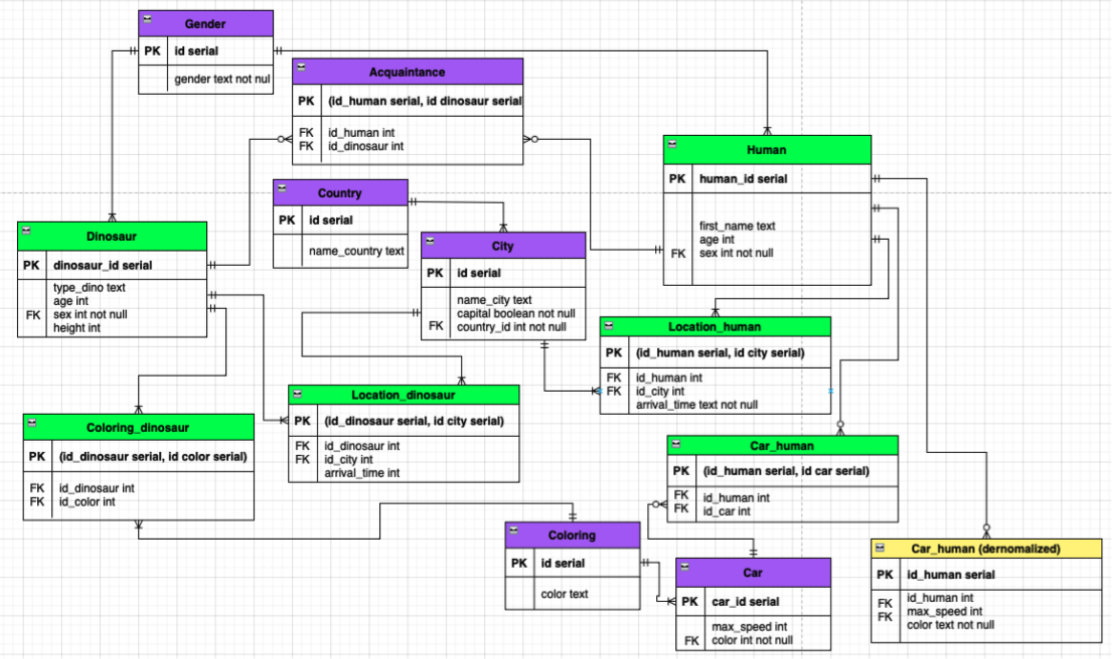
\includegraphics[width=.9\textwidth]{123}